

\tikzset{every picture/.style={line width=0.75pt}} %set default line width to 0.75pt        

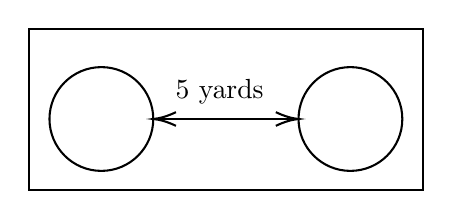
\begin{tikzpicture}[x=0.75pt,y=0.75pt,yscale=-1,xscale=1]
%uncomment if require: \path (0,235); %set diagram left start at 0, and has height of 235

%Shape: Circle [id:dp44350233650848403] 
\draw   (250,136) .. controls (250,122.19) and (261.19,111) .. (275,111) .. controls (288.81,111) and (300,122.19) .. (300,136) .. controls (300,149.81) and (288.81,161) .. (275,161) .. controls (261.19,161) and (250,149.81) .. (250,136) -- cycle ;
%Shape: Circle [id:dp7540662310947368] 
\draw   (370,136) .. controls (370,122.19) and (381.19,111) .. (395,111) .. controls (408.81,111) and (420,122.19) .. (420,136) .. controls (420,149.81) and (408.81,161) .. (395,161) .. controls (381.19,161) and (370,149.81) .. (370,136) -- cycle ;
%Straight Lines [id:da5895379960576028] 
\draw    (302,136) -- (368,136) ;
\draw [shift={(370,136)}, rotate = 180] [color={rgb, 255:red, 0; green, 0; blue, 0 }  ][line width=0.75]    (10.93,-3.29) .. controls (6.95,-1.4) and (3.31,-0.3) .. (0,0) .. controls (3.31,0.3) and (6.95,1.4) .. (10.93,3.29)   ;
\draw [shift={(300,136)}, rotate = 0] [color={rgb, 255:red, 0; green, 0; blue, 0 }  ][line width=0.75]    (10.93,-3.29) .. controls (6.95,-1.4) and (3.31,-0.3) .. (0,0) .. controls (3.31,0.3) and (6.95,1.4) .. (10.93,3.29)   ;
%Shape: Rectangle [id:dp0919307770262141] 
\draw   (240,92.5) -- (430,92.5) -- (430,170) -- (240,170) -- cycle ;


% Text Node
\draw (332,123) node   [align=left] {5 yards};


\end{tikzpicture}
